\documentclass[t]{beamer} 
\usepackage{tikz}
\usepackage[all]{xy}
\usepackage{amsmath,amssymb}
\usepackage{hyperref}
\usepackage{graphicx}
\usepackage[noend]{algcompatible}
\usepackage{multirow}

\DeclareMathOperator*{\argmin}{arg\,min}
\DeclareMathOperator*{\Lik}{Lik}
\DeclareMathOperator*{\PoissonLoss}{PoissonLoss}
\DeclareMathOperator*{\Peaks}{Peaks}
\DeclareMathOperator*{\Segments}{Segments}
\DeclareMathOperator*{\argmax}{arg\,max}
\DeclareMathOperator*{\maximize}{maximize}
\DeclareMathOperator*{\minimize}{minimize}
\newcommand{\sign}{\operatorname{sign}}
\newcommand{\RR}{\mathbb R}
\newcommand{\ZZ}{\mathbb Z}
\newcommand{\NN}{\mathbb N}
\newcommand{\z}{$z = 2, 4, 3, 5, 1$} 

\newcommand{\algo}[1]{\textcolor{#1}{#1}}
\definecolor{PDPA}{HTML}{66C2A5}
\definecolor{CDPA}{HTML}{FC8D62}
\definecolor{GPDPA}{HTML}{4D4D4D}

% Set transparency of non-highlighted sections in the table of
% contents slide.
\setbeamertemplate{section in toc shaded}[default][100]
\AtBeginSection[]
{
  \setbeamercolor{section in toc}{fg=red} 
  \setbeamercolor{section in toc shaded}{fg=black} 
  \begin{frame}
    \tableofcontents[currentsection]
  \end{frame}
}

\begin{document}

\title{Optimizing ROC Curves with a Sort-Based Surrogate Loss for Binary Classification and Changepoint Detection, arXiv:2107.01285}

\author{
  Toby Dylan Hocking --- toby.hocking@nau.edu\\ 
  joint work with my student Jonathan Hillman\\
  Machine Learning Research Lab --- \url{http://ml.nau.edu}\\
  School of Informatics, Computing and Cyber Systems\\
  Northern Arizona University, USA\\
  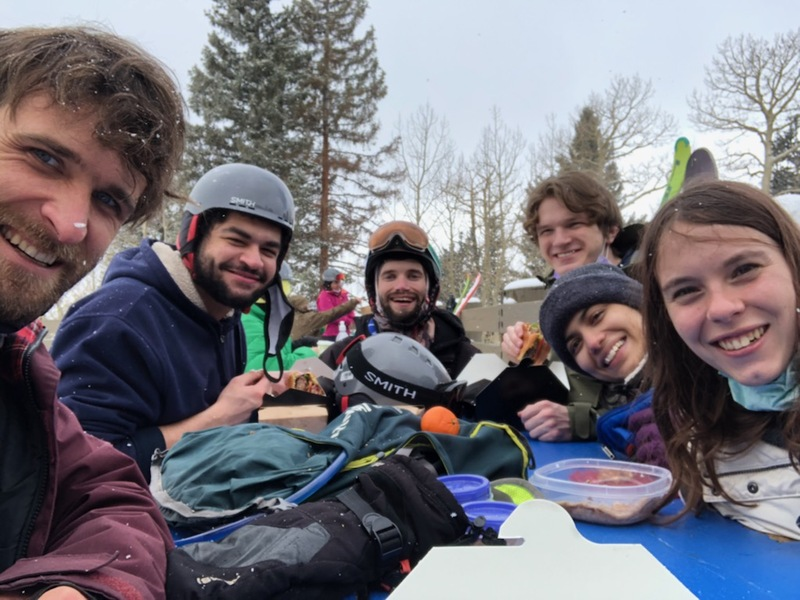
\includegraphics[height=3.5cm]{2021-03-lab-ski-lunch} \\
}

\date{}

\maketitle

\section{Problem Setting 1: ROC curves for evaluating supervised  binary classification algorithms}

\begin{frame}
  \frametitle{Problem: supervised binary classification}
  
  \begin{itemize}
  \item Given pairs of inputs $\mathbf x\in\mathbb R^p$ and outputs
    $y\in\{0,1\}$ can we learn a score 
    $f(\mathbf x)\in\mathbb R$, predict $y=1$ when $f(\mathbf x)>0$?
  \item Example: email, $\mathbf x =$bag of words, $y=$spam or not.
  \item Example: images. Jones {\it et al.} PNAS 2009.
    \parbox{2in}{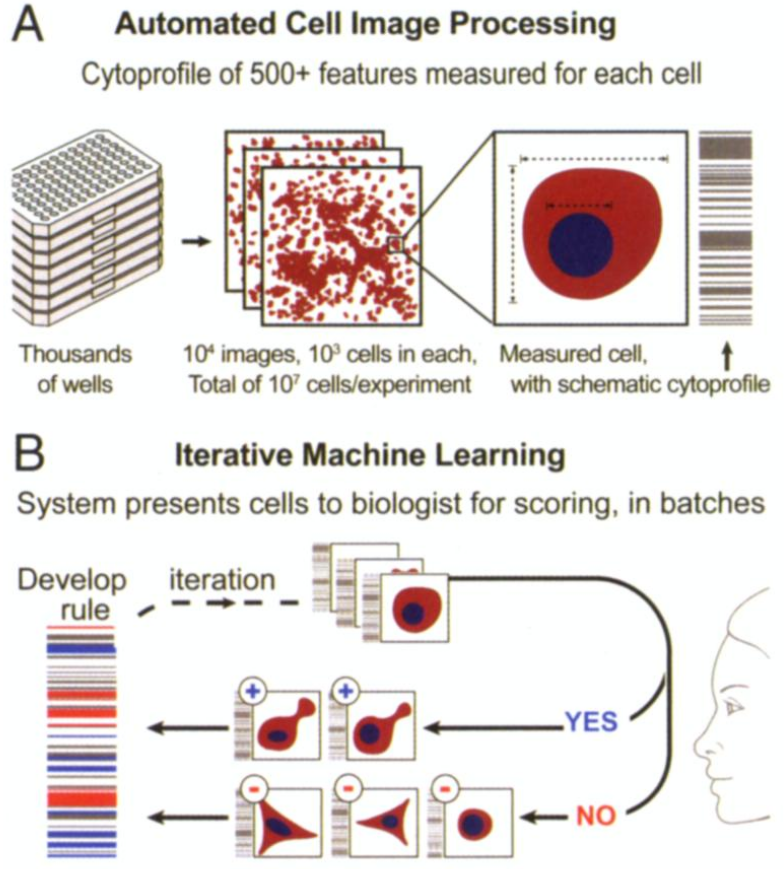
\includegraphics[width=2in]{cellprofiler}}
    \parbox{1.9in}{Most algorithms (SVM, Logistic regression, etc) minimize a differentiable surrogate of zero-one loss = sum of:\\
      \textbf{False positives:} $f(\mathbf x)>0$ but $y=0$ (predict
      budding, but cell is not).\\
      \textbf{False negatives:} $f(\mathbf x)<0$ but $y=1$ (predict
      not budding but cell is).  }
  \end{itemize} 
\end{frame}

\begin{frame}
  \frametitle{Receiver Operating Characteristic (ROC) Curves}
  \begin{itemize}
  \item Classic evaluation method from the signal processing
    literature (Egan and Egan, 1975).
  \item For a given set of predicted scores, plot True Positive Rate
    vs False Positive Rate, each point on the ROC curve is a different
    threshold of the predicted scores.
  \item Best classifier has a point near upper left (TPR=1, FPR=0), with large
    Area Under the Curve (AUC).
  % \item Proposed idea: a new surrogate for AUC that is differentiable,
  %   so can be used for gradient descent learning.
  \end{itemize}
  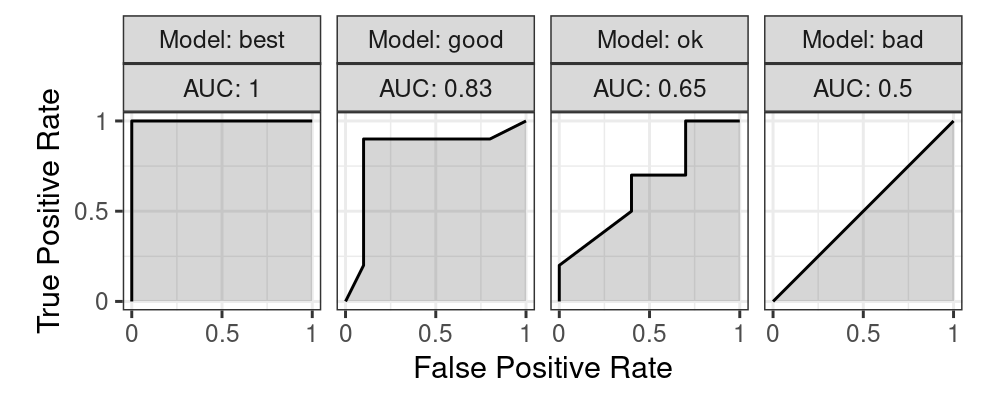
\includegraphics[width=\textwidth]{figure-more-than-one-binary}
\end{frame}

\begin{frame}
  \frametitle{Research question and new idea}
  Can we learn a binary classification function $f$ which directly
  optimizes the ROC curve?
  \begin{itemize}
  \item Most algorithms involve minimizing a differentiable surrogate
    of the zero-one loss, which is not the same.
  \item The Area Under the ROC Curve (AUC) is piecewise constant
    (gradient zero almost everywhere), so can not be used with
    gradient descent algorithms.
  \item We propose to encourage points to be in the upper left of ROC
    space, using a loss function which is a differentiable surrogate
    of the sum of min(FP,FN).
  \end{itemize}
  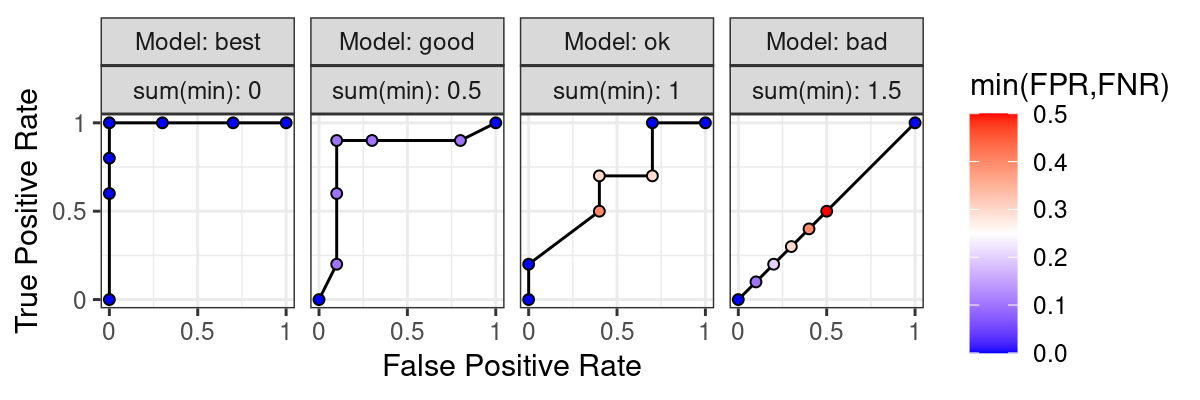
\includegraphics[width=\textwidth]{figure-more-than-one-binary-dots}
\end{frame}
 
\section{Problem setting 2: ROC curves for evaluating supervised changepoint algorithms}

\begin{frame}
  \frametitle{Problem: unsupervised changepoint detection}
  \begin{itemize}
  \item Data sequence $z_1,\dots,z_T$ at $T$ points over time/space.
  \item Ex: DNA copy number data for cancer diagnosis, $z_t\in\mathbb R$.
  \item The penalized changepoint problem (Maidstone \emph{et al.} 2017)
$$\argmin_{u_1,\dots,u_T\in\mathbb R} \sum_{t=1}^T (u_t - z_t)^2 + \lambda\sum_{t=2}^T I[u_{t-1} \neq u_t].$$
  \end{itemize}

  \parbox{0.6\textwidth}{
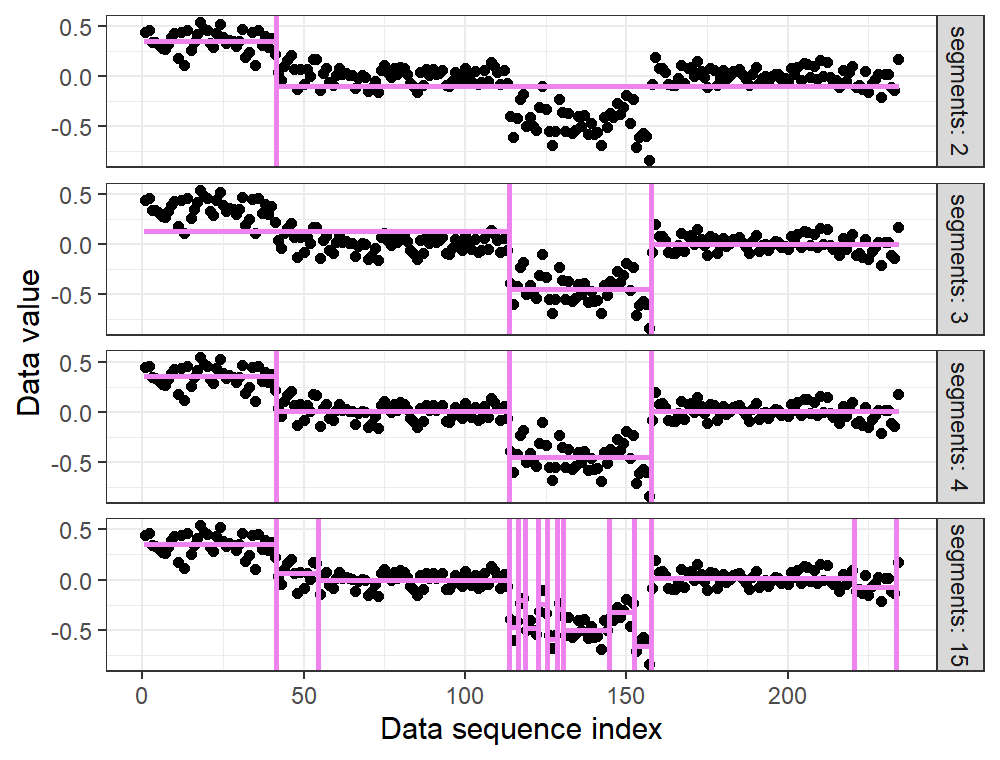
\includegraphics[width=0.6\textwidth]{figure-fn-not-monotonic-no-labels}
}
\parbox{0.3\textwidth}{
  Larger penalty $\lambda$ results in fewer changes/segments.

  \vskip 0.5in

  Smaller penalty $\lambda$ results in more changes/segments.
}

\end{frame}


\begin{frame}
  \frametitle{Problem: weakly supervised changepoint detection}
  \begin{itemize}
  \item First described by Hocking \emph{et al.} ICML 2013.
  \item We are given a data sequence $\mathbf z$ with labeled regions
    $L$.
  \item \alert<2>{We compute features $\mathbf x=\phi(\mathbf z)\in\mathbf R^p$
    and want to learn a function $f(\mathbf x)=-\log\lambda\in\mathbf R$ that minimizes label error (sum of false positives and false negatives), or maximizes AUC.}
  \end{itemize}

  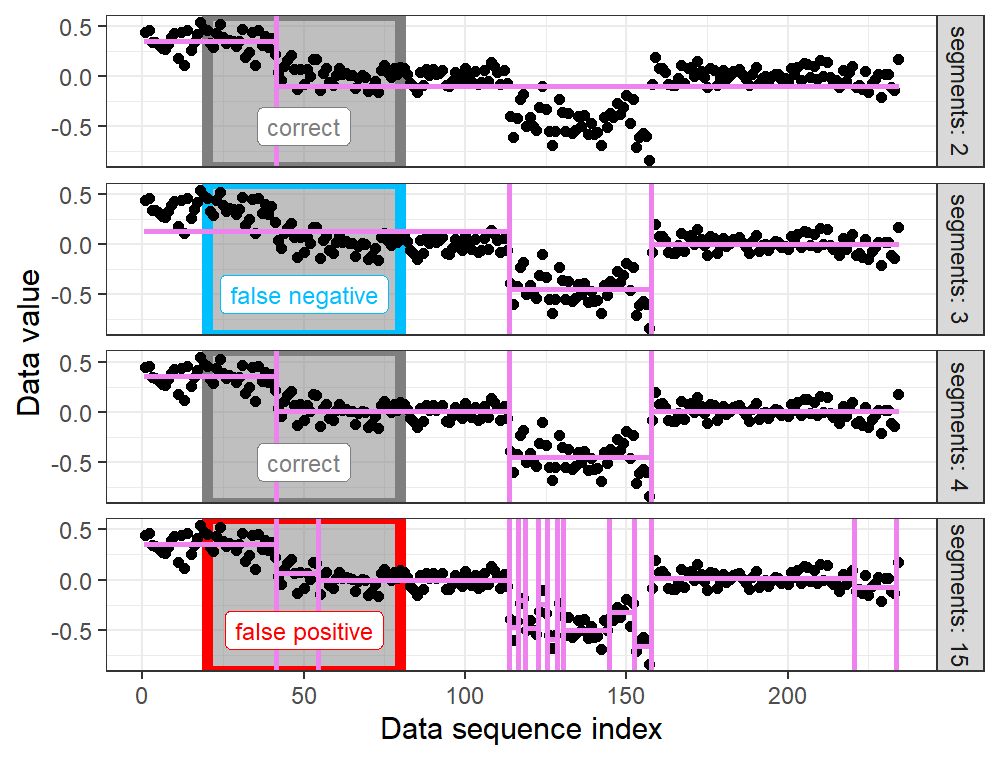
\includegraphics[width=0.56\textwidth]{figure-fn-not-monotonic}
  \only<2>{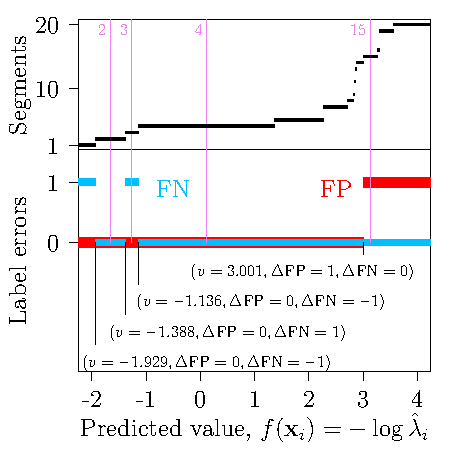
\includegraphics[width=0.42\textwidth]{figure-fn-not-monotonic-error-standAlone}}

\end{frame}

\begin{frame}
  \frametitle{Comparing changepoint algorithms using ROC curves}
  {\scriptsize Hocking TD, Srivastava A. Labeled Optimal Partitioning. Accepted in Computational Statistics, arXiv:2006.13967.}
  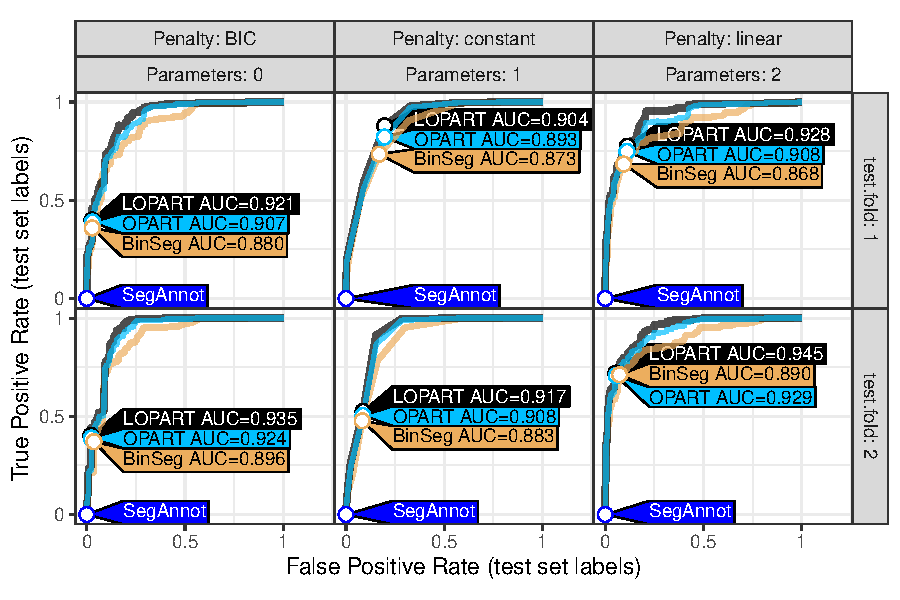
\includegraphics[width=0.9\textwidth]{figure-LOPART-roc}

  LOPART algorithm (R package LOPART) has consistently larger
  test AUC than previous algorithms.
\end{frame}

\section{Proposed surrogate loss for ROC curve optimization: Area Under Min\{FP,FN\} (AUM)} 

\begin{frame}
  \frametitle{Algorithm inputs: predictions and label error functions}

  \begin{itemize}
  \item Each observation $i\in\{1,\dots,n\}$ has a predicted value
    $\hat y_i\in\mathbb R$.
  \item Breakpoints
  $b\in\{1,\dots, B\}$ used to represent label error via tuple
  $(v_b, \Delta\text{FP}_b, \Delta\text{FN}_b, \mathcal I_b)$.
\item There are changes $\Delta\text{FP}_b, \Delta\text{FN}_b$ at
  predicted value $v_b\in\mathbb R$ in error function
  $\mathcal I_b\in\{1,\dots,n\}$.
  \end{itemize}

  \parbox{0.49\textwidth}{
    Binary classification\\
  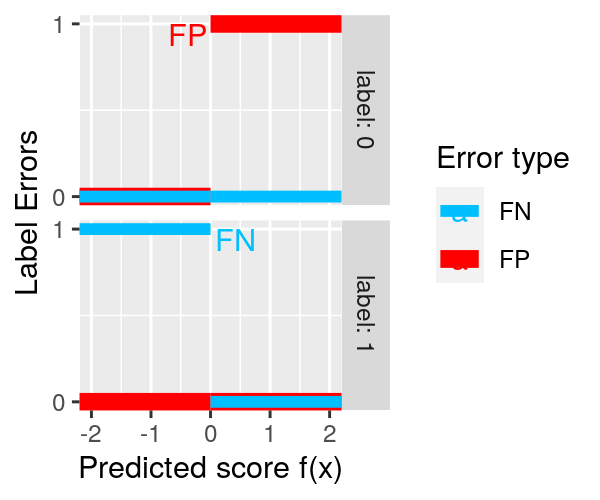
\includegraphics[width=0.49\textwidth]{figure-more-than-one-binary-errors}
}\parbox{0.49\textwidth}{
  Changepoint detection\\
  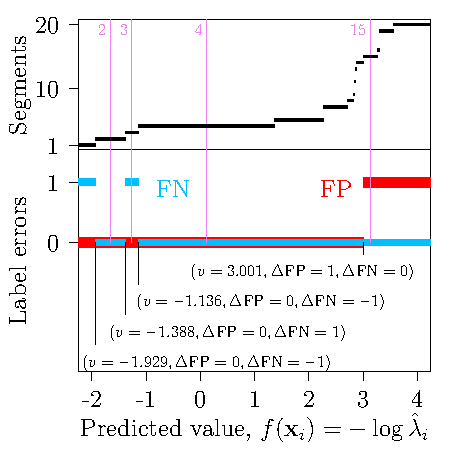
\includegraphics[width=0.49\textwidth]{figure-fn-not-monotonic-error-standAlone}}

\end{frame}

\begin{frame}
  \frametitle{Proposed surrogate loss, Area Under Min (AUM)}
  \begin{itemize}
  \item Threshold
    $t_b= v_b - \hat y_{\mathcal I_b}=\tau(\mathbf{\hat y})_q$ is largest constant you can add to predictions and still be on ROC point $q$.
  \item Proposed surrogate loss, Area Under Min (AUM) of total FP/FN,
    computed via sort and modified cumsum:
  \end{itemize}
\begin{eqnarray*}
  \underline{\text{FP}}_b &=& \sum_{j: t_j < t_b} \Delta\text{FP}_j,\ 
  \overline{\text{FP}}_b = \sum_{j: t_j \leq t_b} \Delta\text{FP}_j, \\
  \underline{\text{FN}}_b &=& \sum_{j: t_j \geq t_b} - \Delta\text{FN}_j,\ 
  \overline{\text{FN}}_b = \sum_{j: t_j > t_b} - \Delta\text{FN}_j.
\end{eqnarray*}

  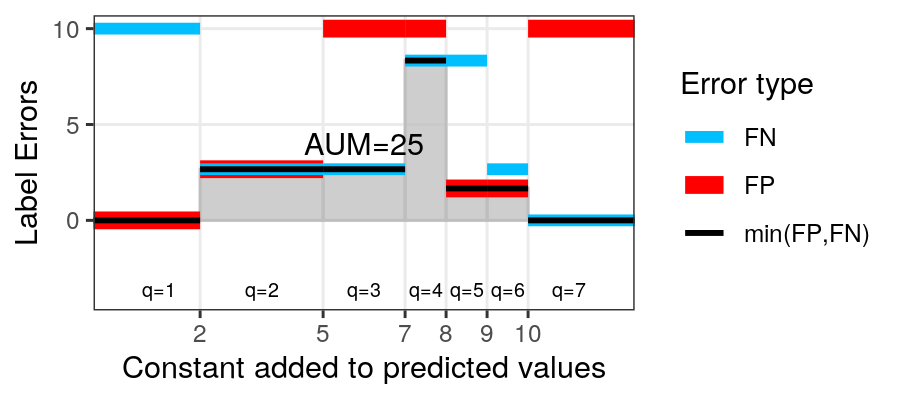
\includegraphics[height=1.5in]{figure-more-than-one-more-aum}
  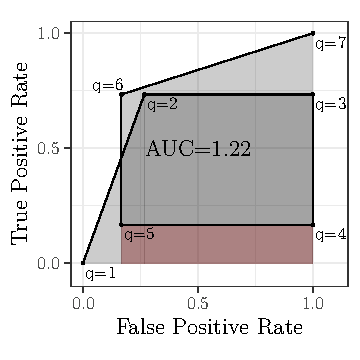
\includegraphics[height=1.5in]{figure-more-than-one-more-auc}

\end{frame}

\begin{frame}
  \frametitle{Small AUM is correlated with large AUC} 
  
  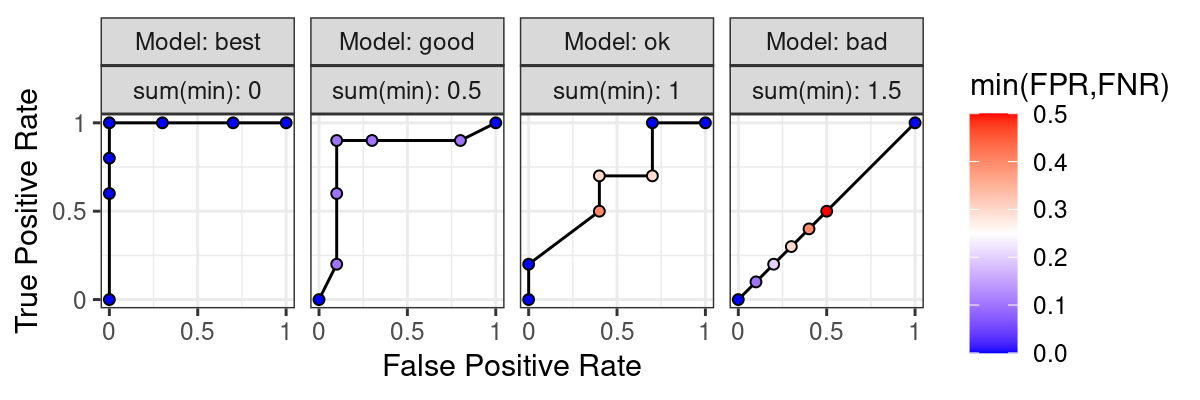
\includegraphics[height=1.5in]{figure-more-than-one-binary-dots}

  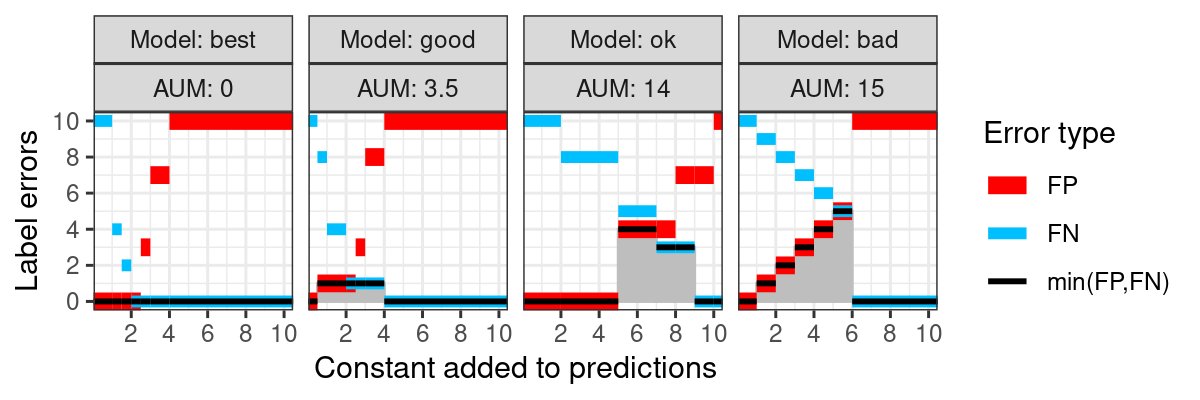
\includegraphics[height=1.5in]{figure-more-than-one-binary-aum}
  
\end{frame}

\begin{frame}
  \frametitle{Proposed algorithm computes two directional derivatives }

  \begin{itemize}
  \item Gradient only defined when function is differentiable, but AUM
    is not differentiable everywhere (see below).
  \item Directional derivatives always computable (R package aum),
  \end{itemize}
% \begin{theorem}
% \label{thm:directional-derivs}
% The AUM directional derivatives for a particular example
% $i\in\{1,\dots,n\}$ can be computed using the following equations.
% \end{theorem}
\begin{eqnarray*}
  &&\nabla_{\mathbf v(-1,i)} \text{AUM}(\mathbf{\hat y}) = \\
  &&\sum_{b: \mathcal I_b = i}
  \min\{
  \overline{\text{FP}}_b , 
  \overline{\text{FN}}_b 
  \}
  -
  \min\{
  \overline{\text{FP}}_b - \Delta\text{FP}_b, 
  \overline{\text{FN}}_b - \Delta\text{FN}_b
  \},\\
  &&\nabla_{\mathbf v(1,i)} \text{AUM}(\mathbf{\hat y}) = \\
  &&\sum_{b: \mathcal I_b = i}
  \min\{
  \underline{\text{FP}}_b + \Delta\text{FP}_b, 
  \underline{\text{FN}}_b + \Delta\text{FN}_b
  \}
  -
  \min\{
  \underline{\text{FP}}_b , 
  \underline{\text{FN}}_b 
     \}.
\end{eqnarray*}  

\parbox{2in}{ 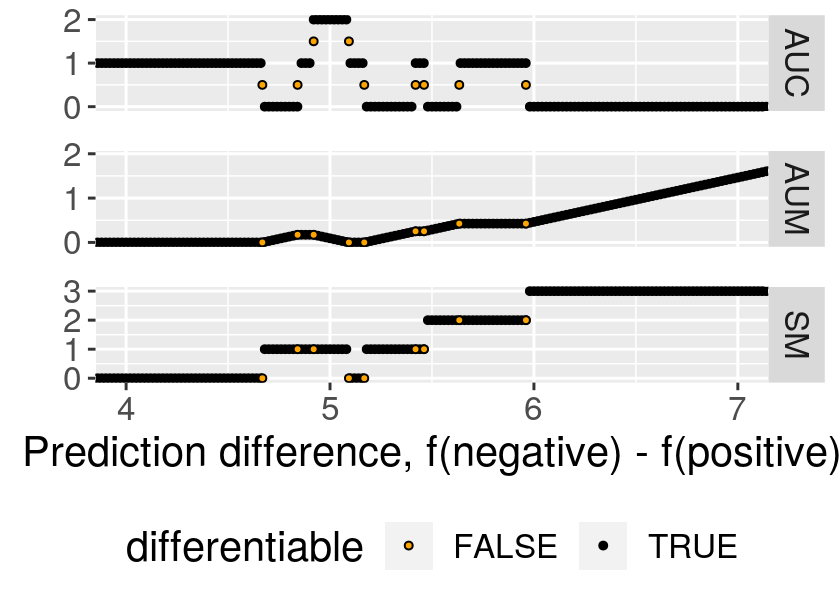
\includegraphics[width=2in]{figure-aum-convexity} }
\parbox{2in}{ Proposed learning algo uses mean of these two
  directional derivatives as ``gradient.''  }

\end{frame}

\section{Empirical results: minimizing AUM results in optimized ROC curves}

\begin{frame}
  \frametitle{AUM gradient descent results in increased train AUC for
    a real changepoint problem}

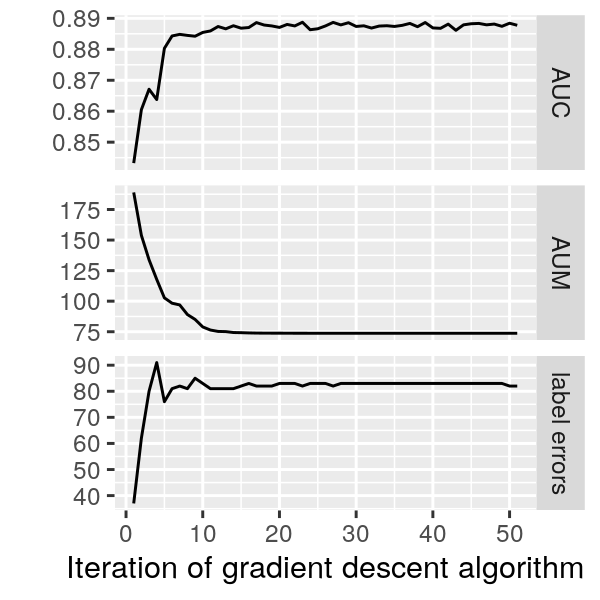
\includegraphics[height=3.7cm]{figure-aum-optimized-iterations.png}
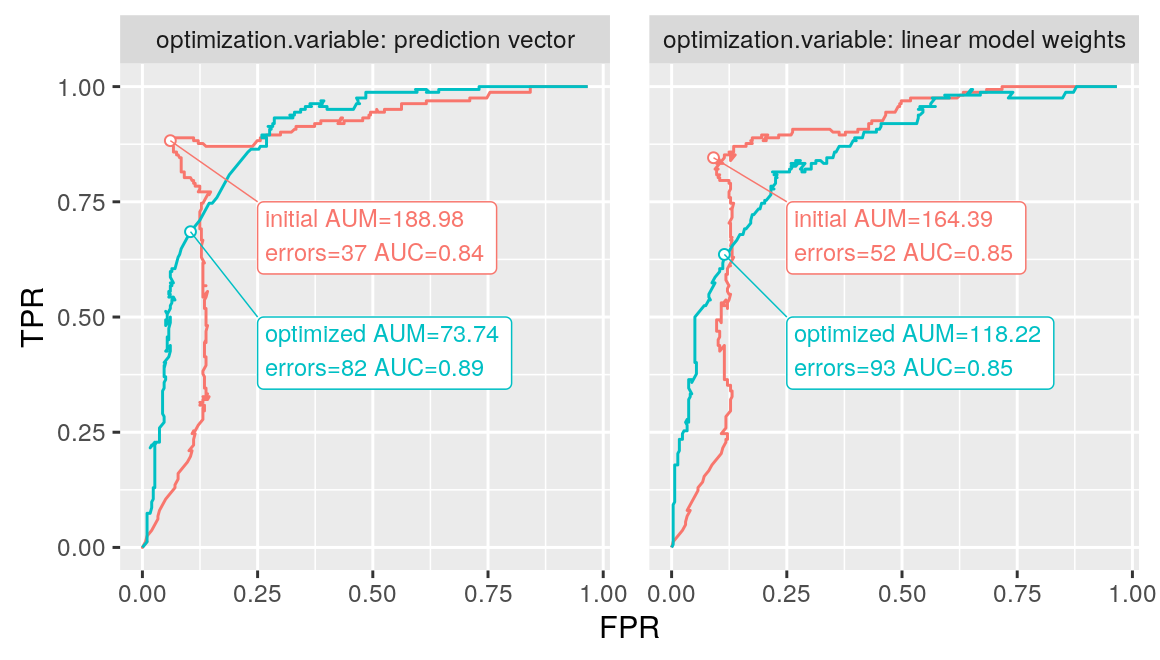
\includegraphics[height=3.7cm]{figure-aum-train-both.png}

\begin{itemize}
\item Left/middle: changepoint problem initialized to prediction vector with
  min label errors, gradient descent on prediction vector.
\item Right: linear model initialized by minimizing regularized convex
  loss (surrogate for label error, Hocking \emph{et al.} ICML 2013),
  gradient descent on weight vector.
\end{itemize}

\end{frame}

\begin{frame}
  \frametitle{Learning algorithm results in better test AUC/AUM for changepoint problems}
    
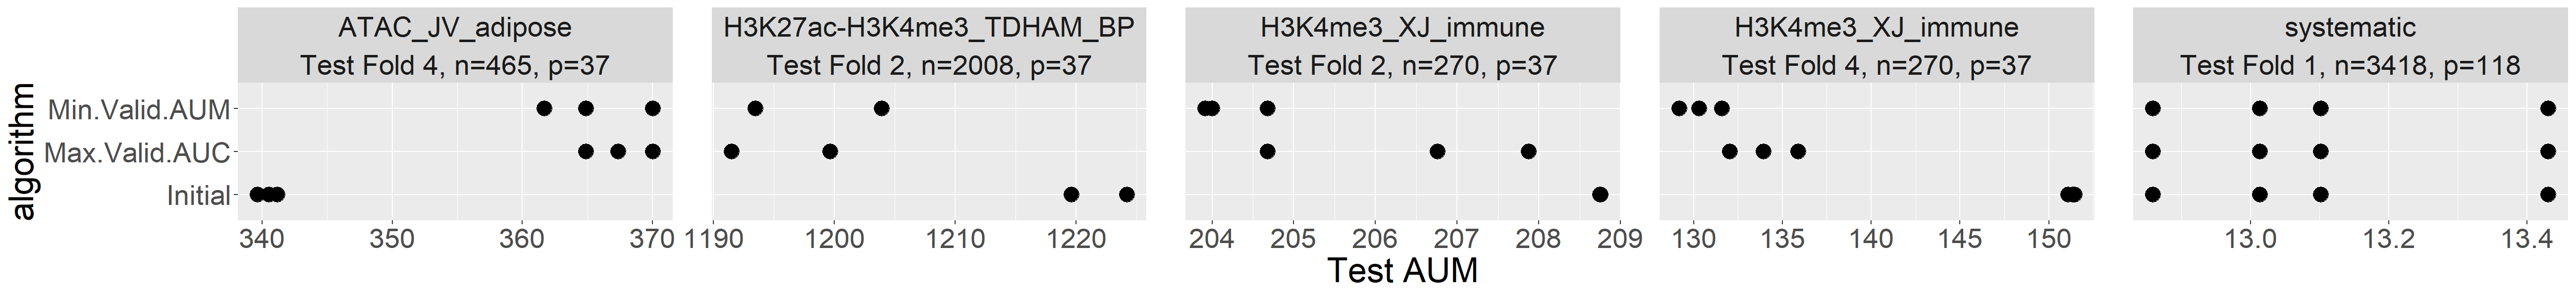
\includegraphics[width=\textwidth]{figure-test-aum-comparison.png}
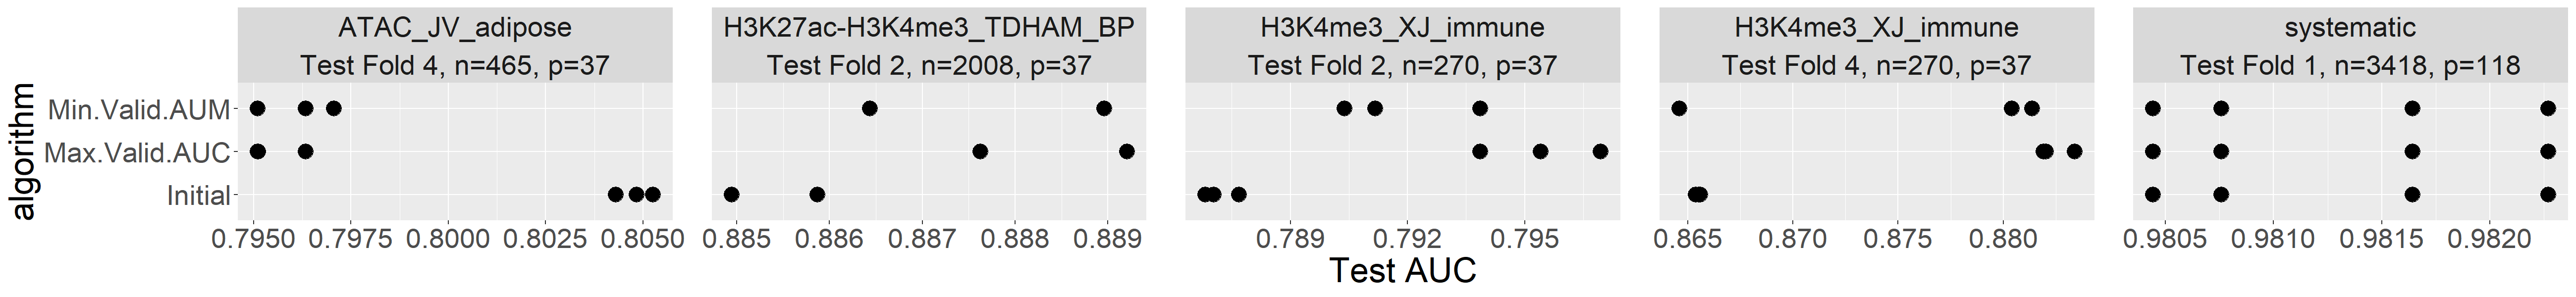
\includegraphics[width=\textwidth]{figure-test-auc-comparison.png}

\begin{itemize}
\item Five changepoint problems (panels from left to right).
\item Two evaluation metrics (AUM=top, AUC=bottom).
\item Three algorithms (Y axis), Initial=Min regularized convex loss
  (surrogate for label error, Hocking \emph{et al.} ICML 2013), Min.Valid.AUM/Max.Valid.AUC=AUM
  gradient descent with early stopping regularization.
\item Four points = Four random initializations.
\end{itemize}

\end{frame}

\begin{frame}
  \frametitle{Learning algorithm competitive for unbalanced binary classification}

 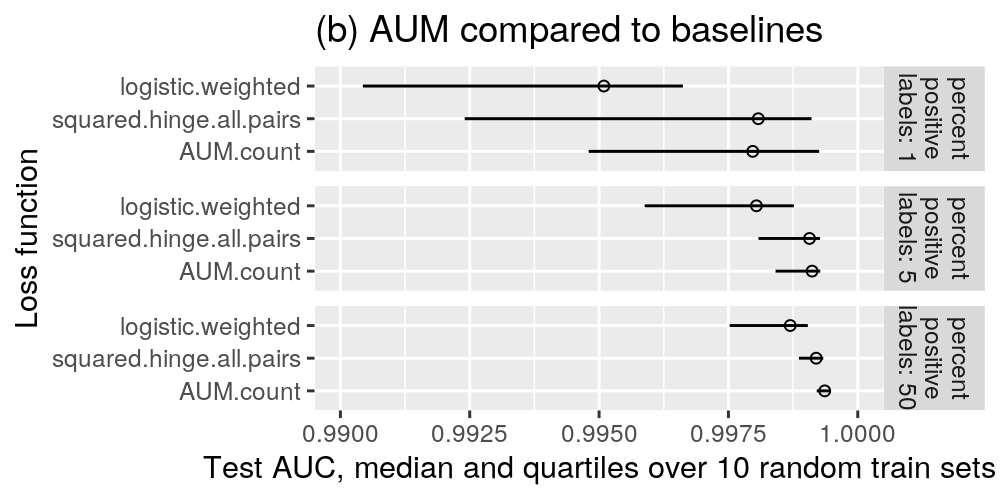
\includegraphics[width=\textwidth]{figure-unbalanced-grad-desc.png}

 \begin{itemize}
 \item Squared hinge all pairs is a classic/popular surrogate loss function
   for AUC optimization. (Yan \emph{et al.} ICML 2003)
 \item All linear models with early stopping regularization.
 \end{itemize}

\end{frame}

\section{Discussion and Conclusions}

\begin{frame}
  \frametitle{Discussion and Conclusions, Pre-print arXiv:2107.01285}
  \begin{itemize}
  \item ROC curves are used to evaluate binary classification and
    changepoint detection algorithms.
  % \item In changepoint detection there can be loops in ROC curves, so
  %   maximizing AUC greater than 1 is not be desirable.
  % \item In changepoint detection, maximizing Area Under ROC curve is
  %   non-trivial even for the train set with unconstrained
  %   predictions.
  \item We propose a new loss function, AUM=Area Under Min(FP,FN),
    which is a differentiable surrogate of the sum of Min(FP,FN) over
    all points on the ROC curve.
  \item We propose new algorithm for efficient AUM and directional
    derivative computation.
  \item Implementations available in R and python/torch:
    \url{https://cloud.r-project.org/web/packages/aum/}
    \url{https://tdhock.github.io/blog/2022/aum-learning/}
  \item Empirical results provide evidence that learning using AUM
    minimization results in ROC curve optimization (encourages
    monotonic/regular curves with large AUC).
  \item Future work: exploiting piecewise linear structure of the AUM
    loss, other model classes, other problems/objectives.
  \end{itemize}
\end{frame}

\begin{frame}
  \frametitle{Thanks to co-author Jonathan Hillman! (second from left)}

  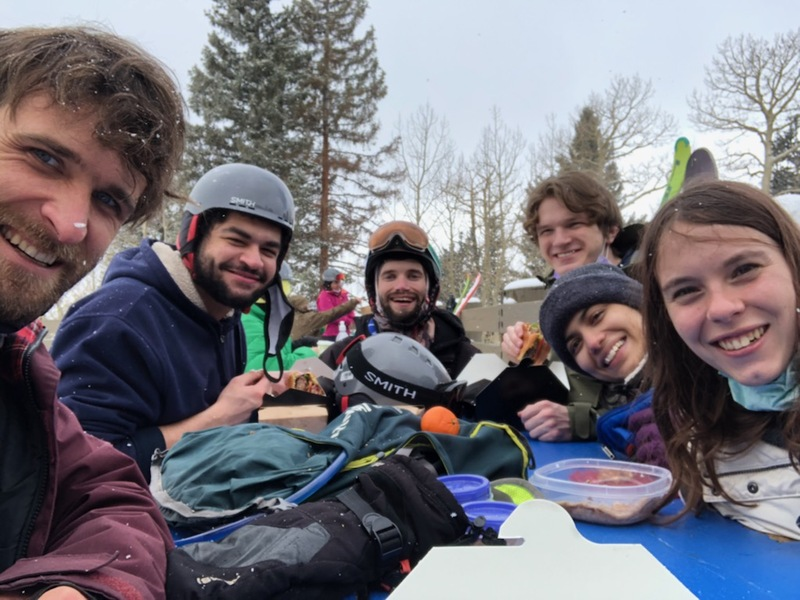
\includegraphics[height=3in]{2021-03-lab-ski-lunch} 

  Contact: toby.hocking@nau.edu

\end{frame} 

\end{document}
